\documentclass[border=10pt]{standalone}
\usepackage[T1]{fontenc}
\usepackage{tikz}
\usepackage[svgnames]{xcolor}
\usetikzlibrary{shapes.geometric, arrows.meta, positioning, calc}

\colorlet{OrangeFill}{LightSalmon}
\colorlet{OrangeLine}{DarkSalmon!30!Chocolate}
\colorlet{GreenFill}{MediumAquamarine}
\colorlet{GreenLine}{MediumAquamarine!30!Teal}
\colorlet{PurpleFill}{MediumPurple}
\colorlet{PurpleLine}{MediumPurple!30!SlateBlue}
\colorlet{PinkFill}{Thistle}
\colorlet{PinkLine}{Thistle!30!Plum}
\colorlet{BlueFill}{LightSkyBlue}
\colorlet{BlueLine}{SteelBlue}
\colorlet{GrayFill}{LightGray!60!OldLace}
\colorlet{GrayLine}{RosyBrown!50!Silver}

\begin{document}
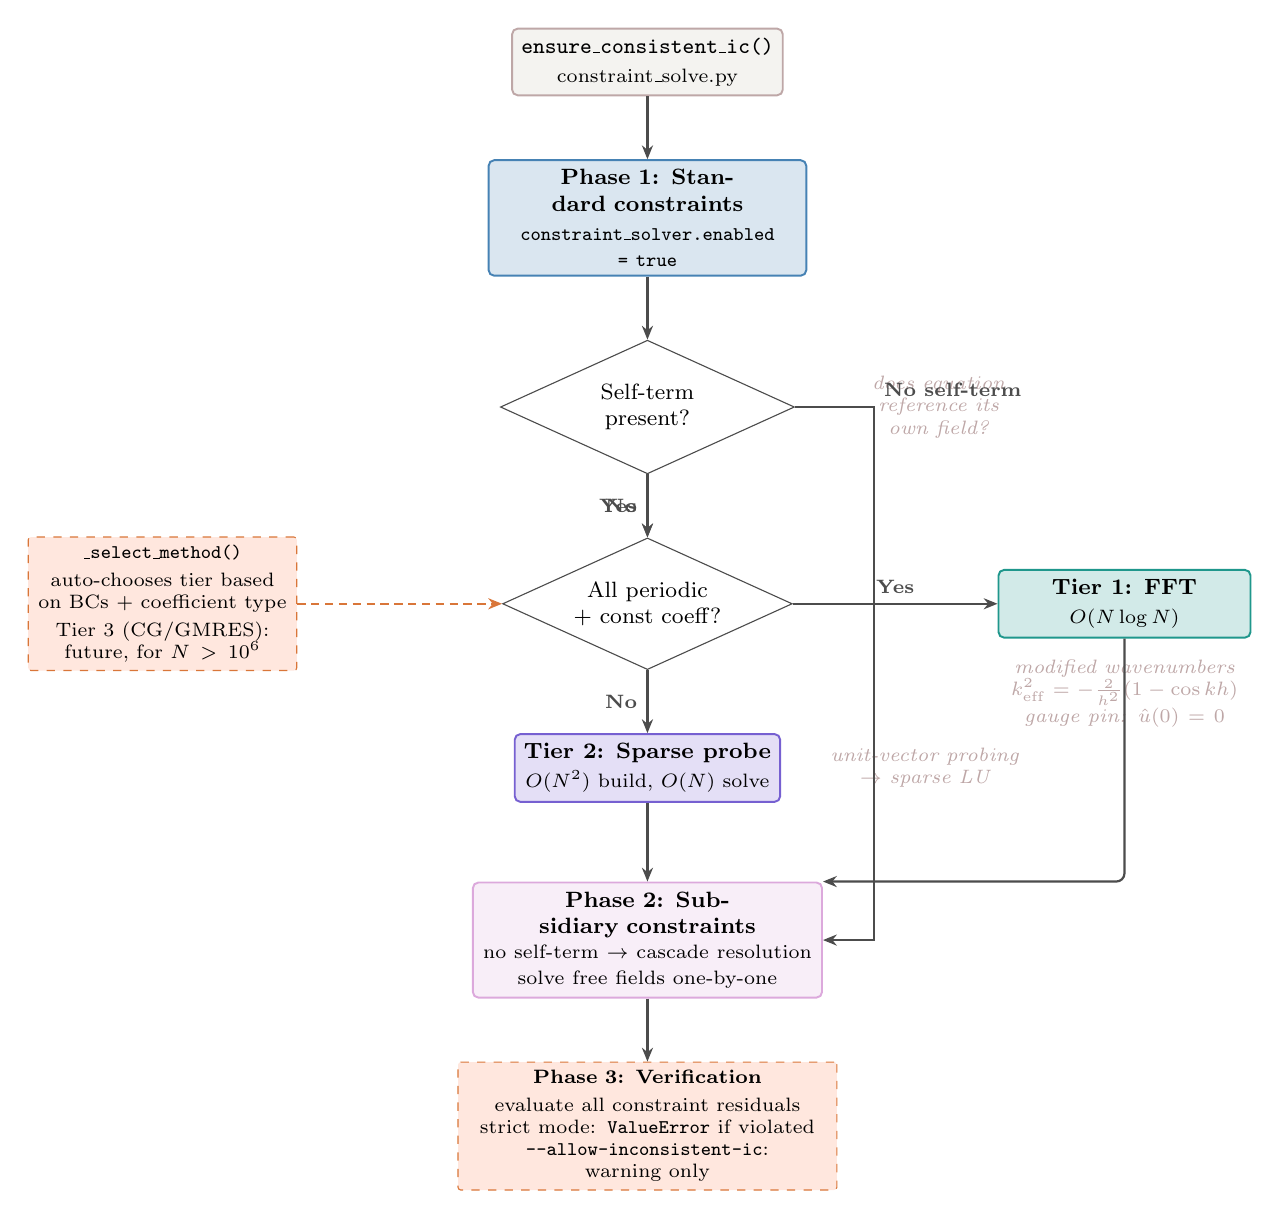
\begin{tikzpicture}[
    decision/.style={
        diamond, aspect=2.2, minimum width=1.6cm,
        draw=black!70, fill=white, font=\footnotesize,
        align=center, inner sep=2pt, text width=2.0cm
    },
    stage/.style={
        rectangle, rounded corners=2pt, minimum width=3.2cm,
        minimum height=0.8cm, draw=#1, line width=0.7pt,
        fill=#1!20, font=\footnotesize, align=center,
        text opacity=1, text=black
    },
    stage/.default={black!70},
    check/.style={
        rectangle, rounded corners=1pt, draw=OrangeLine, dashed,
        fill=OrangeFill, fill opacity=0.25, font=\scriptsize,
        align=center, text opacity=1, inner sep=3pt
    },
    annot/.style={font=\scriptsize\itshape, text=GrayLine, align=center,
                  text width=3.0cm},
    arr/.style={-{Stealth[length=5pt, width=4pt]}, thick, black!70},
    yeslbl/.style={font=\scriptsize\bfseries, text=black!70},
    nolbl/.style={font=\scriptsize\bfseries, text=black!70},
    node distance=0.8cm and 2.6cm
]

% ===================================================================
% ENTRY
% ===================================================================
\node[stage=GrayLine, fill=GrayFill, fill opacity=0.4] (entry)
    {\textbf{\texttt{ensure\_consistent\_ic()}}\\[1pt]
     \scriptsize constraint\_solve.py};

% ===================================================================
% PHASE 1: Standard constraints
% ===================================================================
\node[stage=BlueLine, below=0.8cm of entry, text width=3.8cm] (ph1)
    {\textbf{Phase 1: Standard constraints}\\[1pt]
     \scriptsize \texttt{constraint\_solver.enabled = true}};

\node[decision, below=0.8cm of ph1] (d1)
    {Self-term\\present?};

\node[annot, right=0.2cm of d1.east, anchor=west]
    {does equation\\reference its\\own field?};

% Tier selection
\node[decision, below=0.8cm of d1] (d2)
    {All periodic\\+ const coeff?};

% Tier 1
\node[stage=GreenLine, right=2.6cm of d2] (t1)
    {\textbf{Tier 1: FFT}\\[1pt]
     \scriptsize $O(N \log N)$};
\node[annot, below=0.15cm of t1]
    {modified wavenumbers\\$k_{\mathrm{eff}}^2 = -\frac{2}{h^2}(1-\cos kh)$\\
     gauge pin: $\hat{u}(0)=0$};

% Tier 2
\node[stage=PurpleLine, below=0.8cm of d2] (t2)
    {\textbf{Tier 2: Sparse probe}\\[1pt]
     \scriptsize $O(N^2)$ build, $O(N)$ solve};
\node[annot, right=0.2cm of t2.east, anchor=west]
    {unit-vector probing\\$\to$ sparse LU};

% ===================================================================
% PHASE 2: Iterative propagation
% ===================================================================
\node[stage=PinkLine, below=1.0cm of t2, text width=4.2cm] (ph2)
    {\textbf{Phase 2: Subsidiary constraints}\\[1pt]
     \scriptsize no self-term $\to$ cascade resolution\\
     \scriptsize solve free fields one-by-one};

% ===================================================================
% PHASE 3: Verification
% ===================================================================
\node[check, below=0.8cm of ph2, text width=4.6cm] (ph3)
    {\textbf{Phase 3: Verification}\\[2pt]
     evaluate all constraint residuals\\
     strict mode: \texttt{ValueError} if violated\\
     \texttt{--allow-inconsistent-ic}: warning only};

% ===================================================================
% ARROWS
% ===================================================================
\draw[arr] (entry) -- (ph1);
\draw[arr] (ph1) -- (d1);
\draw[arr] (d1) -- node[nolbl, left] {No} (d2);
\draw[arr] (d1.east) -- ++(1.0,0) |- (ph2.east)
    node[pos=0.0, above right, font=\scriptsize\bfseries] {No self-term};

% Self-term present → tier selection
\draw[arr] (d1) -- node[yeslbl, left] {Yes} (d2);

\draw[arr] (d2) -- node[yeslbl, above] {Yes} (t1);
\draw[arr] (d2) -- node[nolbl, left] {No} (t2);

% Tiers feed into phase 2
\draw[arr, rounded corners=3pt] (t1.south) |- (ph2.north east);
\draw[arr] (t2) -- (ph2);

\draw[arr] (ph2) -- (ph3);

% ===================================================================
% METHOD SELECTION BOX
% ===================================================================
\node[check, left=2.6cm of d2, text width=3.2cm] (selmethod) {%
    \texttt{\_select\_method()}\\[2pt]
    auto-chooses tier based\\
    on BCs + coefficient type\\[2pt]
    Tier 3 (CG/GMRES):\\
    future, for $N > 10^6$};
\draw[arr, densely dashed, OrangeLine] (selmethod) -- (d2);

\end{tikzpicture}
\end{document}
